\documentclass{article}\usepackage[]{graphicx}\usepackage[]{color}
%% maxwidth is the original width if it is less than linewidth
%% otherwise use linewidth (to make sure the graphics do not exceed the margin)
\makeatletter
\def\maxwidth{ %
  \ifdim\Gin@nat@width>\linewidth
    \linewidth
  \else
    \Gin@nat@width
  \fi
}
\makeatother

\definecolor{fgcolor}{rgb}{0.345, 0.345, 0.345}
\newcommand{\hlnum}[1]{\textcolor[rgb]{0.686,0.059,0.569}{#1}}%
\newcommand{\hlstr}[1]{\textcolor[rgb]{0.192,0.494,0.8}{#1}}%
\newcommand{\hlcom}[1]{\textcolor[rgb]{0.678,0.584,0.686}{\textit{#1}}}%
\newcommand{\hlopt}[1]{\textcolor[rgb]{0,0,0}{#1}}%
\newcommand{\hlstd}[1]{\textcolor[rgb]{0.345,0.345,0.345}{#1}}%
\newcommand{\hlkwa}[1]{\textcolor[rgb]{0.161,0.373,0.58}{\textbf{#1}}}%
\newcommand{\hlkwb}[1]{\textcolor[rgb]{0.69,0.353,0.396}{#1}}%
\newcommand{\hlkwc}[1]{\textcolor[rgb]{0.333,0.667,0.333}{#1}}%
\newcommand{\hlkwd}[1]{\textcolor[rgb]{0.737,0.353,0.396}{\textbf{#1}}}%

\usepackage{framed}
\makeatletter
\newenvironment{kframe}{%
 \def\at@end@of@kframe{}%
 \ifinner\ifhmode%
  \def\at@end@of@kframe{\end{minipage}}%
  \begin{minipage}{\columnwidth}%
 \fi\fi%
 \def\FrameCommand##1{\hskip\@totalleftmargin \hskip-\fboxsep
 \colorbox{shadecolor}{##1}\hskip-\fboxsep
     % There is no \\@totalrightmargin, so:
     \hskip-\linewidth \hskip-\@totalleftmargin \hskip\columnwidth}%
 \MakeFramed {\advance\hsize-\width
   \@totalleftmargin\z@ \linewidth\hsize
   \@setminipage}}%
 {\par\unskip\endMakeFramed%
 \at@end@of@kframe}
\makeatother

\definecolor{shadecolor}{rgb}{.97, .97, .97}
\definecolor{messagecolor}{rgb}{0, 0, 0}
\definecolor{warningcolor}{rgb}{1, 0, 1}
\definecolor{errorcolor}{rgb}{1, 0, 0}
\newenvironment{knitrout}{}{} % an empty environment to be redefined in TeX

\usepackage{alltt}
\usepackage{geometry}
\usepackage{amsmath}
\usepackage{lscape}
\geometry{verbose,tmargin=2.5cm,bmargin=2.5cm,lmargin=2.5cm,rmargin=2.5cm}
\IfFileExists{upquote.sty}{\usepackage{upquote}}{}
\begin{document}




\title{Messina E1: The effect of margin on robustness}
\maketitle


%%%%%%%%%%%%%%%%%%%%%%%%%%%%%%%%%%%%%%%%%%%%%%%%%%%%%%%%%%%%%%%%%%%%%%
% LIBRARIES
%%%%%%%%%%%%%%%%%%%%%%%%%%%%%%%%%%%%%%%%%%%%%%%%%%%%%%%%%%%%%%%%%%%%%%
\section{Preparation}
\begin{knitrout}
\definecolor{shadecolor}{rgb}{0.969, 0.969, 0.969}\color{fgcolor}\begin{kframe}
\begin{alltt}
\hlkwd{library}\hlstd{(ggplot2)}
\end{alltt}


{\ttfamily\noindent\itshape\color{messagecolor}{\#\# Loading required package: methods}}\begin{alltt}
\hlkwd{library}\hlstd{(plyr)}
\hlkwd{library}\hlstd{(reshape2)}
\end{alltt}
\end{kframe}
\end{knitrout}


\begin{knitrout}
\definecolor{shadecolor}{rgb}{0.969, 0.969, 0.969}\color{fgcolor}\begin{kframe}
\begin{alltt}
\hlcom{# I need to show: That higher margin leads to greater robustness}
\hlcom{# to high sigma_delta and sigma_epsilon.}

\hlcom{# Define margin as the distance between the 5% error bounds for both 0 and 1.}
\hlstd{deltaForMargin} \hlkwb{=} \hlkwa{function}\hlstd{(}\hlkwc{margin}\hlstd{,} \hlkwc{sigma_epsilon} \hlstd{=} \hlnum{1}\hlstd{,} \hlkwc{alpha} \hlstd{=} \hlnum{0.05}\hlstd{) margin} \hlopt{-} \hlnum{2}\hlopt{*}\hlstd{sigma_epsilon}\hlopt{*}\hlkwd{qnorm}\hlstd{(alpha)}
\hlstd{marginForDelta} \hlkwb{=} \hlkwa{function}\hlstd{(}\hlkwc{delta}\hlstd{,} \hlkwc{sigma_epsilon} \hlstd{=} \hlnum{1}\hlstd{,} \hlkwc{alpha} \hlstd{=} \hlnum{0.05}\hlstd{) delta} \hlopt{+} \hlnum{2}\hlopt{*}\hlstd{sigma_epsilon}\hlopt{*}\hlkwd{qnorm}\hlstd{(alpha)}

\hlstd{e1aii.design} \hlkwb{=} \hlkwd{expand.grid}\hlstd{(}
        \hlkwc{snr} \hlstd{=} \hlkwd{seq}\hlstd{(}\hlnum{0}\hlstd{,} \hlnum{5}\hlstd{,} \hlnum{0.1}\hlstd{),}
\hlcom{#	p1 = c(0.2, 0.5, 0.8),		# Result is independent of p1}
        \hlkwc{p1} \hlstd{=} \hlnum{0.5}\hlstd{,}
        \hlkwc{sigma_epsilon} \hlstd{=} \hlnum{1}\hlstd{,}
        \hlkwc{sigma_delta} \hlstd{=} \hlkwd{seq}\hlstd{(}\hlnum{0}\hlstd{,} \hlnum{2}\hlstd{,} \hlnum{1}\hlstd{),}
        \hlkwc{alpha} \hlstd{=} \hlnum{0.1}\hlstd{)}
\hlstd{e1aii.design}\hlopt{$}\hlstd{Delta} \hlkwb{=} \hlstd{e1aii.design}\hlopt{$}\hlstd{snr} \hlopt{*} \hlstd{e1aii.design}\hlopt{$}\hlstd{sigma_epsilon}
\hlstd{e1aii.design}\hlopt{$}\hlstd{margin} \hlkwb{=} \hlkwd{marginForDelta}\hlstd{(e1aii.design}\hlopt{$}\hlstd{Delta, e1aii.design}\hlopt{$}\hlstd{sigma_epsilon,} \hlkwc{alpha} \hlstd{= e1aii.design}\hlopt{$}\hlstd{alpha)}
\hlstd{e1aii.design}\hlopt{$}\hlstd{threshold} \hlkwb{=} \hlstd{e1aii.design}\hlopt{$}\hlstd{Delta}\hlopt{/}\hlnum{2}

\hlstd{e1aii.design}\hlopt{$}\hlstd{error} \hlkwb{=} \hlkwd{unlist}\hlstd{(}\hlkwd{mlply}\hlstd{(e1aii.design,} \hlkwa{function}\hlstd{(}\hlkwc{threshold}\hlstd{,} \hlkwc{p1}\hlstd{,} \hlkwc{Delta}\hlstd{,} \hlkwc{sigma_delta}\hlstd{,} \hlkwc{sigma_epsilon}\hlstd{,} \hlkwc{...}\hlstd{) \{}
        \hlstd{Err_internal} \hlkwb{=} \hlkwa{function}\hlstd{(}\hlkwc{d}\hlstd{) ((}\hlnum{1}\hlopt{-}\hlstd{p1)}\hlopt{*}\hlstd{(}\hlnum{1}\hlopt{-}\hlkwd{pnorm}\hlstd{((threshold} \hlopt{-} \hlstd{d)}\hlopt{/}\hlstd{sigma_epsilon))} \hlopt{+} \hlstd{p1}\hlopt{*}\hlkwd{pnorm}\hlstd{((threshold} \hlopt{-} \hlstd{(Delta} \hlopt{+} \hlstd{d))}\hlopt{/}\hlstd{sigma_epsilon))}
        \hlkwa{if} \hlstd{(sigma_delta} \hlopt{==} \hlnum{0}\hlstd{)   \{}       \hlkwd{return}\hlstd{(}\hlkwd{Err_internal}\hlstd{(}\hlnum{0}\hlstd{)) \}}
        \hlkwa{else} \hlstd{\{}                                          \hlkwd{return}\hlstd{(}\hlkwd{integrate}\hlstd{(}\hlkwa{function}\hlstd{(}\hlkwc{d}\hlstd{)} \hlkwd{Err_internal}\hlstd{(d)} \hlopt{*} \hlnum{1}\hlopt{/}\hlstd{sigma_delta} \hlopt{*} \hlkwd{dnorm}\hlstd{(d} \hlopt{/} \hlstd{sigma_delta),} \hlopt{-}\hlnum{Inf}\hlstd{,} \hlnum{Inf}\hlstd{)}\hlopt{$}\hlstd{value) \}}
\hlstd{\}))}

\hlcom{# + ggtitle("High-margin classifiers are more robust")}
\hlkwd{ggplot}\hlstd{(e1aii.design[e1aii.design}\hlopt{$}\hlstd{margin} \hlopt{>=} \hlnum{0}\hlstd{,],} \hlkwd{aes}\hlstd{(}\hlkwc{x} \hlstd{= margin,} \hlkwc{y} \hlstd{= error,} \hlkwc{colour} \hlstd{=} \hlkwd{factor}\hlstd{(sigma_delta)))} \hlopt{+} \hlkwd{geom_line}\hlstd{(}\hlkwc{lwd} \hlstd{=} \hlnum{1}\hlstd{)} \hlopt{+} \hlkwd{xlab}\hlstd{(}\hlstr{"Margin"}\hlstd{)} \hlopt{+} \hlkwd{ylab}\hlstd{(}\hlstr{"Error rate"}\hlstd{)} \hlopt{+} \hlkwd{labs}\hlstd{(}\hlkwc{colour} \hlstd{=} \hlkwd{expression}\hlstd{(sigma[delta]))} \hlopt{+} \hlkwd{theme_bw}\hlstd{()}
\end{alltt}
\end{kframe}

{\centering 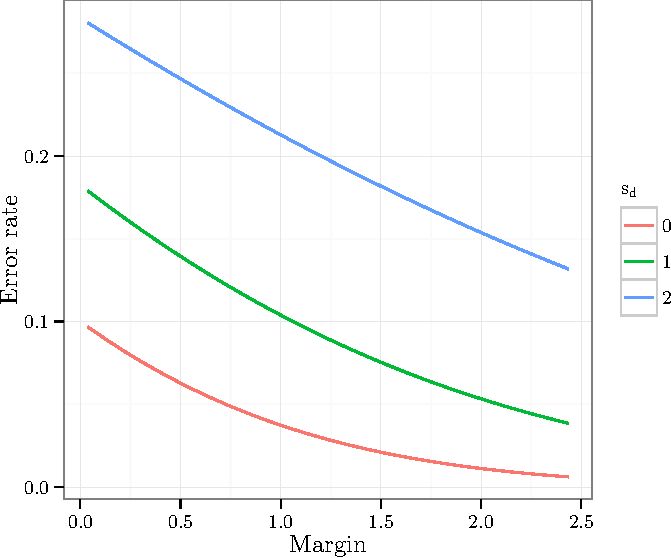
\includegraphics[width=\maxwidth]{figure/05-E1-E1A-1} 

}



\end{knitrout}

\end{document}
